\documentclass{article}

\usepackage[utf8]{inputenc}
\usepackage{amsthm}
\usepackage{amsmath}
\usepackage{amsfonts}
\usepackage{amssymb}
\usepackage{multicol}
\usepackage[polish]{babel}
\usepackage[margin=1.0in]{geometry}
\usepackage[T1]{fontenc}
\usepackage{bbold}
\usepackage{minted}
\usepackage{graphicx}

\newtheorem*{lemma}{Lemat}
\newtheorem*{observation}{Obserwacja}

\let\emptyset\varnothing
\let\leq\leqslant
\let\geq\geqslant

\DeclareMathOperator{\rot}{\mathfrak{r}}
\DeclareMathOperator{\W}{\mathcal{W}}
\DeclareMathOperator{\A}{\mathcal{A}}
\DeclareMathOperator{\Otime}{\mathcal{O}}
\DeclareMathOperator{\states}{\mathcal{S}}
\DeclareMathOperator{\trie}{\mathcal{T}}
\DeclareMathOperator{\goto}{\texttt{goto}}
\DeclareMathOperator{\next}{\texttt{next}}
\DeclareMathOperator{\fail}{\texttt{fail}}
\DeclareMathOperator{\out}{\texttt{output}}
\DeclareMathOperator{\none}{\texttt{None}}

\title{Automat Aho-Corasik\\\large{----- omówienie -----}}
\author{Piotr Mikołajczyk}
\date{}

\begin{document}

\maketitle

% \input{01-intro}
% \input{02-idea}
% \input{03-construction}
% \input{04-analysis}
% \input{05-2d}

\section{Wprowadzenie}

Niech $\W=\{w_1,...,w_k\}$ będzie zbiorem wzorców (niepustych słów nad alfabetem $\Sigma$). Otrzymawszy słowo $T\in\Sigma^n$ chcemy wyznaczyć wszystkie indeksy z $[n]$, na których w $T$ zaczyna się pewien wzorzec z $\W$. Naturalnym rozwiązaniem jest $k$-krotne użycie jednego z wydajnych (liniowych) algorytmów do szukania pojedynczego wzorca. Podejście takie oczywiście jest poprawne, niestety skutkuje złożonością czasową $\Theta(kn)$. Okazuje się, że na podstawie $\W$ jesteśmy w stanie skonstruować w czasie $\Theta(\sum_{i\in[k]}|w_i|)$ odpowiednią strukturę, która będzie potrafiła znaleźć naraz wszystkie wystąpienia wzorców oglądając $T$ wyłącznie raz. Przed nami: automat Aho-Corasick.

\section{Idea}

Pomysł polega na zbudowaniu odpowiedniego deterministycznego automatu skończonego $\A$. Czytając $T$ będziemy podróżować zgodnie z krawędziami $\A$. W każdym stanie $s$ będziemy mieć zapisaną listę tych wzorców z $\W$, które \textit{kończą się} w $s$ -- tzn. aby znaleźć się w stanie $s$ musieliśmy przejść skądś krawędziami etykietowanymi kolejnymi literami pewnego wzorca. Spacerowanie po $\A$ wzdłuż $T$ możemy interpretować jako poruszanie się \textit{jednocześnie} po wszystkich słowach z $\W$.

Zaczniemy konstrukcję od utworzenia \textit{drzewa trie} na podstawie $\W$. Następnie dodamy do każdego stanu informacje o wzorcach które się w nim kończą i podniesiemy funkcję przejścia z częściowej do totalnej. Na koniec uprościmy automat. Po tych zabiegach otrzymamy strukturę, dzięki której wyszukiwanie wielu wzorców okaże się bardzo proste:

\begin{minted}[xleftmargin=20pt,linenos]{python}
def find_occurrences(self, text, n):
  state = self._root
  for i in range(1, n + 1):
    state = state.nxt(text[i])
  for keyword_len in state.output():
    start_pos = i - keyword_len + 1
    yield text[start_pos:i + 1], start_pos
\end{minted}

Warto zwrócić uwagę na fakt, że jeśli dany zbiór wzorców chcemy wyszukać w wielu różnych tekstach $T_1,...,T_t$, to wystarczy tylko raz skonstruować automat Aho-Corasick i użyć go niezależnie na każdym z $T_j$.

\section{Konstrukcja}
\textit{Uwaga: sednem naszych rozważań jest opis sposobu, w jaki można przechodzić pomiędzy stanami automatu. Wygodnie nam będzie utożsamić ze sobą różne podejścia realizacji -- równoważne dla nas będą pojęcia zbioru etykietowanych krawędzi (skierowanych) pomiędzy dwoma stanami, funkcji mapujących pary (stan, symbol) w stan oraz lokalne w stanach tablice routingu.}

\subsection{Drzewo trie}
Mając zbiór słów $\W$ nad alfabetem $\Sigma$ możemy w prosty sposób zbudować tzw. \textit{drzewo trie}, ozn. $\trie_{\W}$. Jest to skierowane, ukorzenione drzewo, którego krawędzie etykietowane są symbolami z $\Sigma$. Każde słowo $w\in\W$ ma odpowiadającą mu ścieżkę z korzenia, etykietowaną kolejnymi literami $w$. Jeśli $w\in\W$ nie jest prefiksem żadnego innego słowa z $\W$, to jego ścieżka kończy się w liściu. Inaczej ujmując, istnieje bijekcja pomiędzy ścieżkami w $\trie_{\W}$ a wszystkimi (różnymi) prefiksami słów z $\W$. Krawędź etykietowaną symbolem $a$ pomiędzy $s_1$ a $s_2$ możemy kodować jako trójkę $(s_1, a, s_2)$.

\begin{figure}[h!]
    \centering
    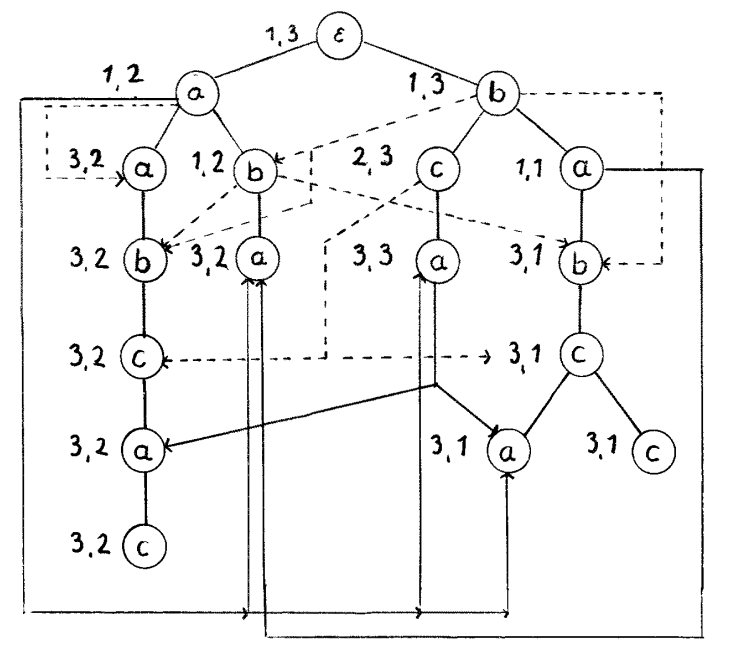
\includegraphics[width=0.4\textwidth]{images/trie.png}
    \caption{$\trie_{\{aaab, aab, bab, ba\}}$}
    \label{fig:trie}
\end{figure}

\subsection{Plan}
Zacznijmy temat konstrukcji od zdefiniowania funkcji, które będą nam potrzebne. Niech $\W$ oznacza zbiór wzorców, $\trie$ oznacza drzewo trie dla $\W$ (skrót dla $\trie_{\W}$), $\rot$ oznacza korzeń $\trie$, $\states$ oznacza zbiór wierzchołków $\trie$ (czyli docelowo zbiór stanów $\A$).

\begin{itemize}
    \item $\goto::\states\times\Sigma\mapsto\states$ -- ta funkcja w zasadzie reprezentuje zbiór krawędzi $\trie$; dodatkowo jednak, dla każdego symbolu w $\Sigma$, który nie etykietuje żadnej krawędzi wychodzącej z $\rot$, dodajemy pętlę w $\rot$; czyli:
    \begin{gather*}
        \goto(s_1, a)=\begin{cases}
        s_2 &\qquad \text{jeśli } (s_1,a,s_2)\in E[\trie] \\
        \rot &\qquad \text{jeśli } s_1=\rot\ \wedge\ \forall_{s}\ (\rot,a,s)\notin E[\trie] \\
        \none
        \end{cases}
    \end{gather*}

    \item $\out::\states\mapsto\wp(\W)$ -- jak zostało już wspomniane, chcemy w każdym stanie $s$ przechowywać listę wzorców, których wystąpienie w $T$ będzie poświadczone odwiedzeniem stanu $s$; w sporym zakresie możemy to obliczyć już przy konstrukcji $\trie$ (np. wracając do rysunku \ref{fig:trie}, $\out(1)=\emptyset$, $\out(5)=\{aab\}$, $\out(7)=\{ba\}$); będziemy musieli jeszcze jednak obsłużyć przypadki, gdy jeden wzorzec będzie sufiksem drugiego (np. $\out(4)=\{aaab, aab\}$)

    \item $\fail::\states\mapsto\states$ -- ostatecznie $\A$ będzie skonstruowane na wierzchołkach $\trie$ więc już teraz możemy spróbować zinterpretować obecność w stanie $s$ po przeczytaniu $j$-tego symbolu $T$ -- otóż etykiety na ścieżce pomiędzy $\rot$ a $s$ tworzą najdłuższy możliwy prefiks któregoś ze wzorców z $\W$, który da się dopasować w $T$ kończąc na pozycji $j$; funkcja $\goto$ jest częściowa, a więc dla niektórych stanów i niektórych symboli nie mamy zdefiniowanego przejścia (na razie otrzymamy $\none$); aby nie utknąć i zachować poprawność interpretacji, to $\fail(s)$ musi wskazywać na taki stan $s'$, żeby słowo powstałe ze ścieżki $\rot\rightsquigarrow s'$ było najdłuższym możliwym sufiksem słowa odpowiadającemu $\rot\rightsquigarrow s$; w dalszej części utożsamiać będziemy ścieżki ze słowami;

    Chodzenie krawędziami $\fail$ opiera się na identycznym pomyśle co rekurencyjne używanie tablic $Border$ w algorytmie Morrisa-Pratta. Warto również zauważyć, że $\fail$ nie ma sensu definiować dla $\rot$.

    \item $\next::\states\times\Sigma\mapsto\states$ -- trzy zdefiniowane funkcje powyżej zupełnie wystarczają, aby nasz docelowy automat robił to, czego pragniemy; jak jednak łatwo zauważyć, próba przeczytania jednego znaku z $T$ może wymagać więcej niż jednego przejścia krawędzią korzystając z $\goto$ oraz $\fail$ -- możemy musieć schodzić wzdłuż $\fail$ wielokrotnie; aby uniknąć tego, pod sam koniec utworzymy funkcję $\next$, która skompresuje nam tego typu ścieżki i zastąpi $\goto$ oraz $\fail$
\end{itemize}

\subsection{Obliczanie $\goto$, $\out$, $\fail$}
Jak już wiemy \textit{co} chcemy policzyć, to możemy przejść do tego \textit{jak} to zrobić. Funkcję $\goto$ oraz część $\out$, jak już zauważyliśmy, możemy obliczyć konstruując $\trie_{\W}$:
\begin{minted}[xleftmargin=20pt,linenos]{python}
def _construct_goto(self, keywords, alphabet):
  for k, k_len in keywords:
    self._enter(k, k_len)

  for a in alphabet:
    if self._root.goto(a) is None:
      self._root.update_goto(a, self._root)

def _enter(self, keyword, keyword_len):
  current_state = self._root
  j = 1

  while j < keyword_len and current_state.goto(keyword[j]) is not None:
    current_state = current_state.goto(keyword[j])
    j += 1

  for a in keyword[j:keyword_len + 1]:
    next_state = AhoCorasickAutomaton.Node()
    current_state.update_goto(a, next_state)
    current_state = next_state

  current_state.append_outputs([(keyword, keyword_len)])
\end{minted}

Funkcja \mintinline{python}{def _enter(...)} uzupełnia częściowo skonstruowane drzewo trie o ścieżkę dla podanego wzorca, w razie potrzeby tworząc nowe węzły. W pętli w wierszu 5. uzupełniamy definicję $\goto$ dla korzenia.

\vspace{10pt}

Funkcję $\fail$ powinniśmy obliczać dla coraz bardziej odległych od $\rot$ węzłów -- podobnie jak w algorytmie Morrisa-Pratta długości najdłuższych borderów obliczaliśmy na podstawie wartości dla krótszych słów:

\begin{minted}[xleftmargin=20pt,linenos]{python}
def _construct_fail(self, alphabet):
  q = Queue()
  for s in (self._root.goto(a) for a in alphabet):
    if s != self._root:
      q.put(s)
      s.update_fail(self._root)

  while not q.empty():
    current = q.get()
    for a, child in ((a, current.goto(a)) for a in alphabet):
      if child is not None:
        q.put(child)

        fallback = current.fail()
        while fallback.goto(a) is None:
          fallback = fallback.fail()

        child_fallback = fallback.goto(a)
        child.update_fail(child_fallback)
        child.append_outputs(child_fallback.output())
\end{minted}

Przechodzimy zatem po $\trie$ za pomocą algorytmu BFS. Będąc w wierzchołku $\texttt{current}$, widząc krawędź etykietowaną przez $\texttt{a}$ do wierzchołka $\texttt{child}$, chcemy obliczyć wartość $\fail(\texttt{child})$. Szukamy więc najdłuższego sufiksu słowa generowanego przez $\rot\rightsquigarrow\texttt{child}$ obecnego w $\trie$. Będzie to najdłuższy sufiks ścieżki $\rot\rightsquigarrow\texttt{current}$, który można przedłużyć o symbol $\texttt{a}$.

Znalazłszy odpowiedni wierzchołek -- $\texttt{child\textunderscore fallback}$ -- powiększamy zbiór $\out(\texttt{child})$ o wartości z  $\out(\texttt{child\textunderscore fallback})$ -- z oczywistej indukcji wynika, że $\out(\texttt{child\textunderscore fallback})$ zawiera już wszystkie wzorce, które są sufiksami $\rot\rightsquigarrow\texttt{child\textunderscore fallback}$.

\subsection{Obliczanie $\next$}

Jeśli $\goto$ była określona dla $s\in\states$ oraz $a\in\Sigma$, to $\next(s, a) = \goto(s, a)$. W przeciwnym wypadku będąc w $s$ i chcąc przejść symbolem $a$, powinniśmy schodzić krawędziami $\fail$ tak długo, aż znajdziemy się w $s'$, dla którego $\goto(s', a)\neq\none$. Jest to podobny zabieg co poprawka Knutha do algorytmu Morrisa-Pratta.
\begin{minted}[xleftmargin=20pt,linenos]{python}
def _construct_next(self, alphabet):
  q = Queue()
  for a in alphabet:
    a_child = self._root.goto(a)
    self._root.update_next(a, a_child)
    if a_child != self._root:
      q.put(a_child)
  self._root.use_only_next()

  while not q.empty():
    current = q.get()
    for a, child in ((a, current.goto(a)) for a in alphabet):
      if child is not None:
        q.put(child)
        current.update_next(a, child)
      else:
        fallback = current.fail()
        current.update_next(a, fallback.next(a))
    current.use_only_next()
\end{minted}

Instrukcje w wierszach 8. oraz 19. pozwalają zwolnić pamięć zapominając o wartościach funkcji $\goto$ i $\fail$. Formalnie dopiero teraz, struktura $\A$ ze zbiorem stanów $\states$ oraz funkcją przejścia $\next$ jest deterministycznym automatem skończonym.

\section{Analiza}
\subsection{Analiza poprawności}
Z tego, co już zostało przedstawione, powinna wynikać poprawność zastosowanej metody. Aby jednak formalnie jej dowieść, wystarczy postawić trzy proste lematy:

\begin{lemma}
Niech $s,t\in\states$ i niech $u, v$ będą słowami generowanymi przez ścieżki $\rot\rightsquigarrow s$ i $\rot\rightsquigarrow t$. Wówczas $\fail(s) = t \iff v$ jest najdłuższym właściwym sufiksem $u$, który jest prefiksem pewnego $w_i\in\W$.
\end{lemma}

\begin{lemma}
Słowo $k$ należy do $\out(s)\iff$ $w\in\W$ oraz $k$ jest sufiksem słowa generowanego przez $\rot\rightsquigarrow s$.
\end{lemma}

\begin{lemma}
Po przeczytaniu $j$ znaków z $T$ znajdujemy się w stanie $s\iff$ słowo generowane przez $\rot\rightsquigarrow s$ jest najdłuższym sufiksem $T[1..j]$, który jest prefiksem pewnego $w\in\W$.
\end{lemma}

\noindent Ich uzasadnienia są prostymi dowodami rekurencyjnymi zapisanymi we fragmentach kodu powyżej.

\subsection{Analiza złożoności}
Konstrukcja całego automatu polega na sekwencyjnym wywołaniu procedur obliczających funkcje przejścia:

\begin{minted}[xleftmargin=20pt,linenos]{python}
class AhoCorasickAutomaton:
  def __init__(self, keywords, alphabet):
    self._root = AhoCorasickAutomaton.Node()
    self._construct_goto(keywords, alphabet)
    self._construct_fail(alphabet)
    self._construct_next(alphabet)
\end{minted}

Niech $m=\max_i |w_i|$. Bardzo łatwo zauważyć, że każdą z powyższych operacji wykonać można w czasie $\Otime(km)$ (dokładnie $\Theta(\sum_{i\in[k]}|w_i|)$) -- za każdym razem przechodzimy po całym drzewie $\trie$ odwiedzając każdy wierzchołek dokładnie raz oraz wykonując $\Theta(1)$ operacji w każdym z nich. Zakładamy również, że łączenie zbiorów $\out$ wykonuje się w czasie stałym (jak np. listy wiązane). Warto dodać, że moc $\Sigma$ wlicza się w zapotrzebowanie (zarówno pamięciowe jak i czasowe) liniowo -- rozmiar grafu jest z góry ograniczony przez $|\Sigma|\cdot km$ (z każdego wierzchołka może wychodzi $|\Sigma|$ krawędzi). Konstrukcja $\A$ oraz wyszukiwanie w $T$ odbywają się w czasie liniowo proporcjonalnym do wielkości $\trie$.

Pozostaje zastanowić się, ile czasu zajmie przeczytanie tekstu $T$ ($|T|=n$) i wypisanie wszystkich wystąpień wzorców. Moc $\Sigma$ traktujemy jak stałą.

Najpierw rozważmy sytuację, w której nie zgłaszamy żadnego wystąpienia wzorca (możemy np. tylko zaznaczyć pozycje $T$ o których wiemy, że na nich coś się kończy):
\begin{itemize}
    \item używając funkcji $\goto$ oraz $\fail$ wykonamy co najwyżej $2n$ przejść w $\A$ -- po przeczytaniu dowolnego symbolu przejdziemy dokładnie raz według funkcji $\goto$ i być może wielokrotnie krawędziami $\fail$; łatwo jednak zaobserwować, że każde przejście $\fail$ skraca odległość z obecnego wierzchołka do $\rot$, a z $\rot$ zawsze można wyjść używając $\goto$; zatem nie możemy przejść krawędziami $\fail$ więcej razy niż przeszliśmy $\goto$;

    można również spojrzeć na to w ten sposób, że przechodząc automatem $\A$ wzdłuż $T$, pamiętamy dwa wskaźniki w $T$ -- słowo pomiędzy nimi to właśnie to, które jest generowane przez ścieżkę z korzenia do obecnego wierzchołka; przejście $\goto$ przesuwa 'prawy' wskaźnik o 1 w prawo, przejście $\fail$ przesuwa 'lewy' wskaźnik o dodatnią liczbę pozycji w prawą, ale na tyle małą by nie przeskoczyć prawego;

    \item używając funkcji $\next$, przy każdym przeczytanym symbolu z $T$ wykonujemy zawsze jedno przejście -- $n$ ruchów
\end{itemize}

Problem może się pojawić, gdy będziemy chcieli wypisywać wszystkie wystąpienia wzorców. Pesymistycznym przykładem jest $\W=\{a,a^2,a^3,...,a^k\}$ oraz $T=a^n$. Liczba wystąpień będzie $\Theta(kn)$. Jednakże, nie jest to wada zastosowanego algorytmu -- każdy inny algorytm zgłaszający wszystkie wystąpienia wzorców musiałby wykonać co najmniej tyle samo pracy.

Zatem możemy określić złożoność czasową wyszukiwania wielu wzorców w tekście za pomocą automatu Aho-Corasick jako liniową w stosunku do sumy długości wszystkich wzorców oraz ilości ich wystąpień.

\section{Zastosowanie do wzorców 2D}
Okazuje się, że bardzo prosto można użyć automatu Aho-Corasick do wyszukiwania wzorców dwuwymiarowych. W skrócie:
\begin{enumerate}
    \item niech $T$ będzie kwadratową tablicą rozmiaru $n^2$, $P$ - kwadratową tablicą rozmiaru $m^2$ o różnych kolumnach, $m < n$
    \item niech $\W$ będzie zbiorem kolumn $P$
    \item automatem Aho-Corasick szukamy $\W$ w każdej z kolumn $T$; jeśli fragment $j$-tej kolumny od indeksu $i$ pokrywa się z $k$-tą kolumną $P$, to niech $T_P[i][j]=k$
    \item algorytmem KMP szukamy w każdym wierszu $T_P$ ciągu $(1,2,...,m)$
\end{enumerate}
Całość działa w czasie liniowym od wielkości wejścia i rozmiaru zbioru z którego pochodzą elementy w $T$ oraz $P$.

\end{document}
